\subsection{2-Opt Moves}

\begin{figure}[h]
\begin{center}
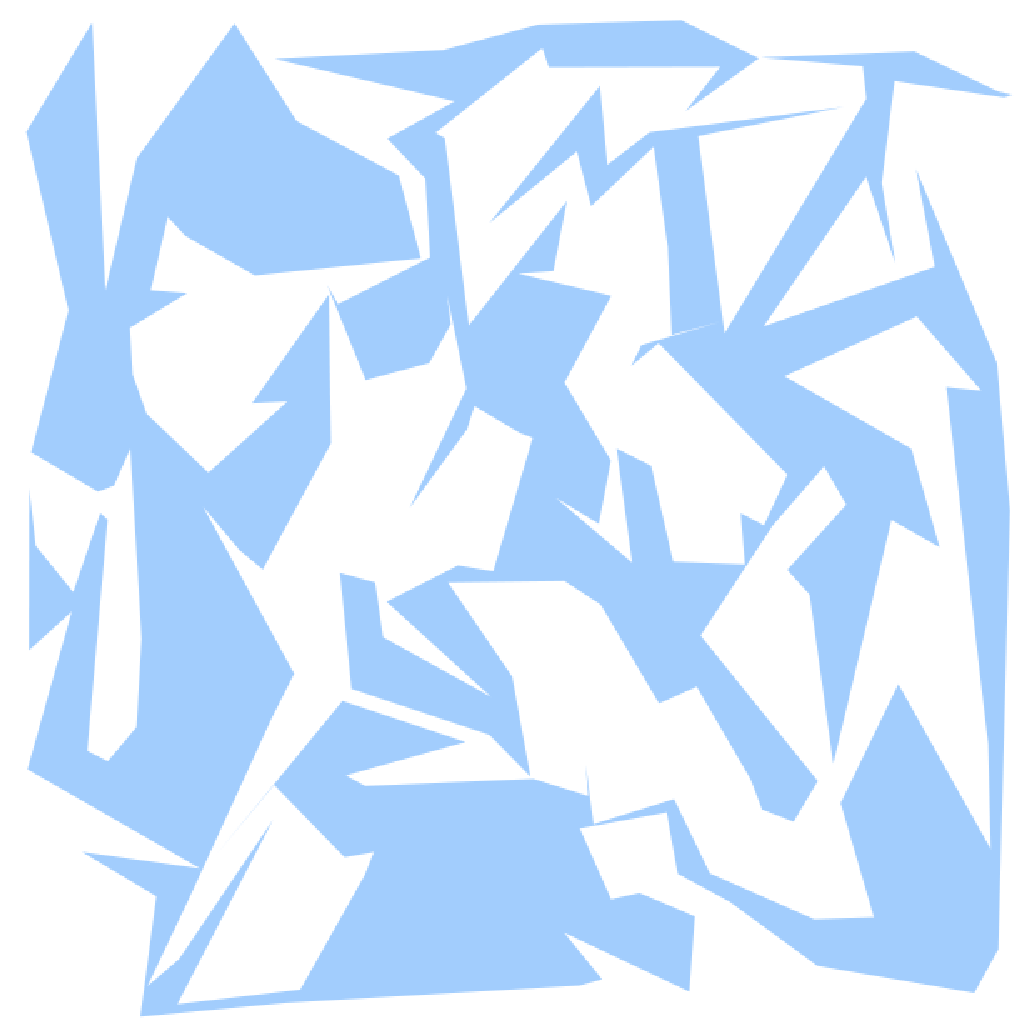
\includegraphics[width=0.3\textwidth]{img/2opt200.eps}
\end{center}
\caption{Polygon mit 200 Punkten (2-Opt Moves)}
\label{fig:2opt200}
\end{figure}

\emph{2-Opt Moves} ist ein einfacher, randomisierter Algorithmus zur Erzeugung von simplen Polygonen, implementiert nach einer Beschreibung von Martin Held in~\cite{held98polygons}. 
\subsubsection{Algorithmus}
Im ersten Schritt des Algorithmus werden die Punkte einer gegebenen Punktmenge zufällig zu einem komplexen Polygon verbunden, ähnlich der Vorgehensweise von \emph{Permute \& Reject}. Anschließend werden die Überschneidungen der Kanten des Polygons mit Hilfe eines sogenannten \enquote{2-opt move} repariert (s. Abbildung~\ref{fig:2optmove}), bis ein überschneidungsfreies Polygon entstanden ist.

\begin{figure}[h]
\begin{center}
\subfigure[Vorher]{
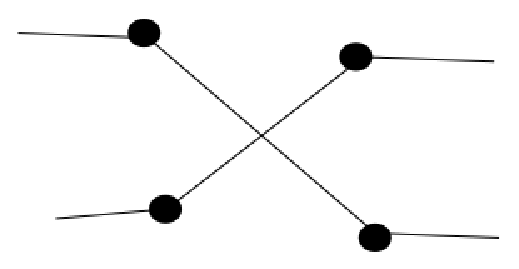
\includegraphics[width=0.4\textwidth]{img/2optbefore.eps}
\label{fig:2optbefore}
}
\subfigure[Nachher]{
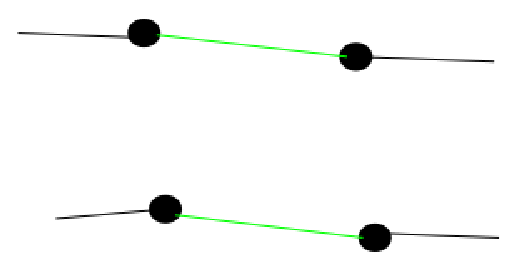
\includegraphics[width=0.4\textwidth]{img/2optafter.eps}
\label{fig:2optafter}
}
\end{center}
\caption{Beispiel eines 2-Opt Move}
\label{fig:2optmove}
\end{figure}

\subsubsection{Eigenschaften}
Laut Held wächst das theoretische Maximum der zur Entfernung aller Schnitte notwendigen 2-Opt moves kubisch mit der Anzahl der gegebenen Punkte, in der Praxis sei die Anzahl der durchgeführten 2-Opt moves jedoch eher quadratisch in Abhängigkeit von $n$. In Verbund mit der von uns implementierten, naiven Polygon-Schnitt-Suche (in $\bigO(n^2)$) erhalten wir ein theoretisches asymptotisches Wachstum der Laufzeit von $\bigO(n^4)$. Da die einzelnen Schritte des Algorithmus jedoch wenig rechenintensiv sind, eignet sich \emph{2-Opt Moves} durchaus zur Konstruktion simpler Polygone mit bis zu 2000 Punkten. Die resultierenden Polygone wirken zudem sehr zufällig und weisen (im Gegensatz bspw. zu \emph{Steady Growth}) keinerlei vorherrschende \enquote{Kantenrichtung} auf.